\begin{mydefs}
	\begin{itemize}
		\iftoggle{eleve}{%
			\item Tous les points \hrulefill
			
			 \vspace*{0.2cm}
			 \hrulefill
			\item Tous les points \hrulefill
			
			\vspace*{0.2cm}
			\hrulefill
		}{%
			\item Tous les points situés à la même distance d'un point $O$, forment un \kw{cercle de centre O}. Cette distance est le \kw{rayon} du cercle.
			\item Tous les points situés à une distance inférieure ou égale = $r$ d'un point $O$, forment ls \kw{disque de centre O} et de rayon $r$.
		}
	\end{itemize}
\end{mydefs}

\begin{myex}
	\begin{multicols}{2}
		
		\begin{itemize}
			\iftoggle{eleve}{%
				\item $O$ est \hrulefill
				\item $[AB]$ est \hrulefill
				\item $[OC]$ est \hrulefill
				\item $[DE]$ est \hrulefill
				
				\vspace*{0.2cm}
				\hrulefill
				\item $A$ \hrulefill
				
				\vspace*{0.2cm}
				\hrulefill
				\item $A$, $O$ et $F$ \hrulefill
				
				\vspace*{0.2cm}
				\hrulefill
			}{%
				\item $O$ est le centre du cercle.
				\item $[AB]$ est un diamètre du cercle.
				\item $[OC]$ est un rayon du cercle.
				\item $[DE]$ est une corde, elle relie deux points du cercle.
				\item $A$ appartient au cercle mais pas $O$, $F$ et $G$.
				\item $A$, $O$ et $F$ appartiennent au disque de centre $O$ et de rayon $OA$, pas $G$.
			}
			
		\end{itemize}
		\begin{center}
			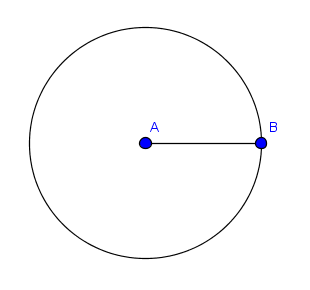
\includegraphics[scale=0.135]{cercle}
		\end{center}
			
	\end{multicols}
\end{myex}

